\documentclass[conference]{IEEEtran}
\IEEEoverridecommandlockouts

% IEEEtran selects Times (ptm). Missing PSNFSS metrics (ptmr7t.tfm) causes
% "Font ... ptmr7t ... not loadable". Install texlive-fonts-recommended for Times;
% otherwise Latin Modern (usually in base TeX) is loaded here.
\IfFileExists{ptmr7t.tfm}{}{%
  \typeout{** Times (ptmr7t.tfm) not found: loading Latin Modern. Install texlive-fonts-recommended for IEEE Times.}%
  \usepackage{lmodern}%
}

% Omit \usepackage{cite} so minimal TeX installs without cite.sty still build.
% For IEEE-style citation sorting/compression, install the `cite` package (e.g.
% texlive-latex-recommended on Debian/Ubuntu) and uncomment the next line.
% \usepackage{cite}
\usepackage{amsmath,amssymb,amsfonts}
\usepackage{graphicx}
\usepackage{textcomp}
\usepackage{url}

% --- Metadata placeholders: replace before submission ---
\newcommand{\PaperTitle}{Vanguard Directions in Deep Learning Models: A Survey Research}
% Uncomment and edit if funding applies:
% \newcommand{\PaperFundingThanks}{This work was supported by ...}

\begin{document}

\title{\PaperTitle\\
}

\author{\IEEEauthorblockN{Alejandro Castro López}
\IEEEauthorblockA{\textit{MNA} \\
\textit{ITESM}\\
a00806170@tec.mx}
\and
\IEEEauthorblockN{Arnulfo Alejandro Cavazos Villarreal}
\IEEEauthorblockA{\textit{MNA} \\
\textit{ITESM}\\
a01796489@tec.mx}
\and
\IEEEauthorblockN{Edmundo Carmona Galindo}
\IEEEauthorblockA{\textit{MNA} \\
\textit{ITESM}\\
a01796647@tec.mx}
\and
\IEEEauthorblockN{Alejandro Castro López}
\IEEEauthorblockA{\textit{MNA} \\
\textit{ITESM}\\
a00806170@tec.mx}
}

\maketitle

\begin{abstract}
This survey-oriented paper synthesizes a set of recent studies that illustrate the leading edge of artificial intelligence research, spanning extreme depth in reinforcement learning, reasoning-centric large language model methods, inference-time scaling and memory efficiency, evaluation of model diversity and homogeneity, and human-centered robot learning. Together these works outline complementary pressures toward more capable systems and toward understanding their limitations, deployment costs, and interaction with users. The discussion is organized around thematic groupings rather than exhaustive coverage of each field, and it foregrounds open questions about scaling, reliability, and responsible use as models and agents become more pervasive.
\end{abstract}

\begin{IEEEkeywords}
Deep learning, large language models, reinforcement learning, reasoning, inference efficiency, human feedback, survey.
\end{IEEEkeywords}

\section{Introduction}
As Artificial Intelligence (AI) models become more prevalent in it's applications both in for end users and developers, it is important to understand the current state of the art and the future directions of the field.
\newline
The following survey covers a brief overview of recent research in the field of deep learning models. The sources used cover a wide range of topics, from scaling depth and reinforcement learning to reasoning, diversity, and evaluation of language models.

\section{Background and terminology}

\paragraph{Attention sinks} Attention sinks are a known failure mode of attention mechanisms in which the attention mechanism becomes saturated and the model becomes unable to attend to new information. This is a problem because it can cause the model to hallucinate or produce incorrect answers.

\paragraph{Chain-of-thought (CoT)} Modern surveys of reasoning-centric language models distinguish \emph{chain-of-thought} (CoT) prompting and training from \emph{reinforced} or preference-tuned variants that treat multi-step reasoning as a policy-learning problem \cite{xu2025reasoning}. Related work also studies \emph{recursive} or dynamically structured CoT, where the model allocates extra reasoning depth where needed rather than using a fixed template \cite{sinha2025drcot}.

\paragraph{Inference-time compute} Across this paper, \emph{inference-time compute} refers to additional forward passes, sampling, or search at deployment, as opposed to parameters updated during training; the \emph{key--value (KV) cache} stores attention states so long contexts and long generations do not recompute full attention from scratch each step.

\paragraph{Preference-based learning} \emph{Preference-based learning} denotes training from ranked options, corrections, or light human signals rather than dense demonstrations.

\section{Scaling depth and reinforcement learning}
Wang \emph{et al.}\ study very deep networks in a self-supervised reinforcement learning setting and report that increasing depth can unlock goal-reaching behaviors that shallower stacks do not exhibit, rather than only improving sample efficiency or final reward by small margins \cite{wang2025thousand}. That framing connects depth to \emph{qualitative} changes in what the agent can represent or plan, not merely to incremental accuracy. Figure~\ref{fig:depth_scaling_rl} summarizes depth scaling in their experiments: deeper models have jumps in performance at certain step thresholds, while shallower models have a more gradual increase or plateau early on. A practical takeaway for survey readers is to separate ``more layers help a little'' from ``depth crosses a threshold where new skills appear''---an empirical question that depends on task structure, representation learning, and optimization, and that motivates careful evaluation beyond aggregate scores.

\begin{figure}[!t]
\centering
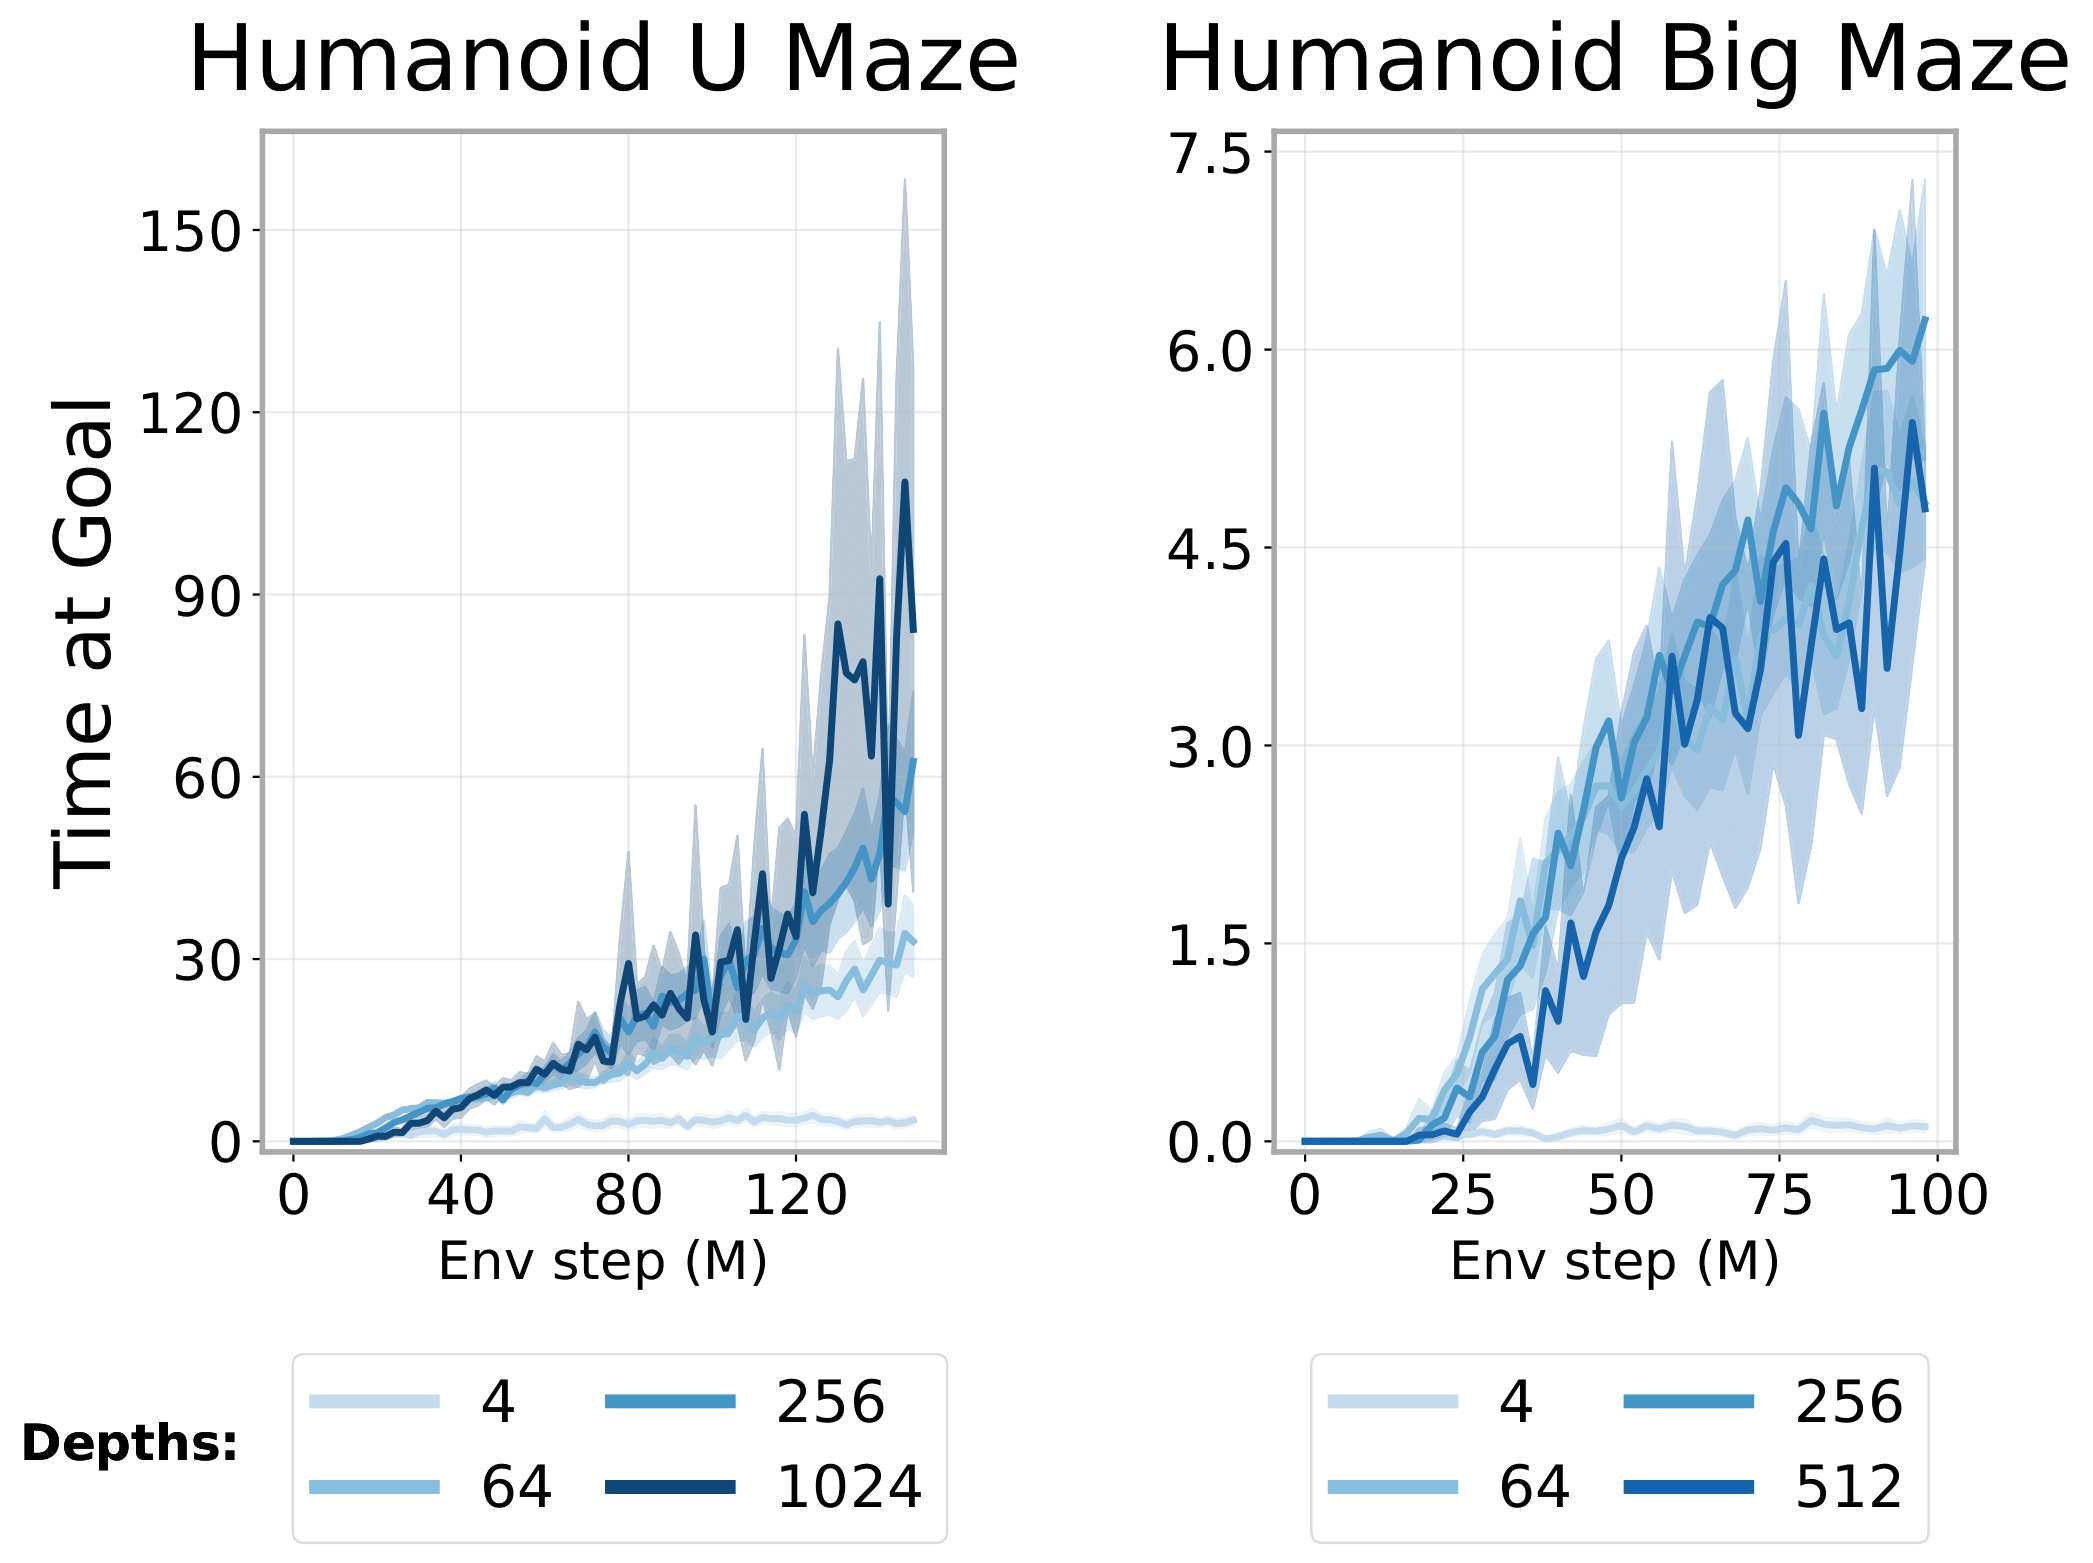
\includegraphics[width=\linewidth]{figures/depth_scaling_limits_2.png}
\caption{Time at goal versus environment steps on Humanoid U Maze (left) and Humanoid Big Maze (right) for policy networks at several depths (lighter to darker blue). Deeper models tend to reach higher time at goal; shaded bands show run-to-run variability. \emph{Reproduced from} \cite{wang2025thousand}.}
\label{fig:depth_scaling_rl}
\end{figure}

\section{Reasoning, diversity, and evaluation of language models}
Complementary work on ``open-ended'' evaluation highlights that many models converge toward similar outputs and failure modes under broad prompts, raising questions about diversity of behavior, dataset design for coverage, and risks when homogeneity interacts with safety-critical deployments \cite{jiang2025hivemind}. Figure~\ref{fig:hivemind} shows the distribution of final answer tokens across models and prompts, highlighting the homogeneity of independently trained models.
Attention variants that gate or reshape softmax behavior aim to improve stability and long-context usability, for example by mitigating known failure modes such as attention sinks and by introducing useful non-linearity or sparsity in the attention map \cite{qiu2025gated}. On the reasoning side, multi-scale CoT fusion aggregates rationales at different granularities to support interpretable, domain-specific chains---Song illustrates this in biological reasoning with large language models, where interpretability and correct structure of the explanation matter alongside the final answer \cite{song2026mscot}. For smaller or parameter-efficient models, dynamic recursive CoT with meta-reasoning offers a way to stretch reasoning capacity without proportionally growing the backbone \cite{sinha2025drcot}. Together these threads show reasoning quality depending on architecture, training, \emph{and} how diversity and failure modes are measured.

\begin{figure}[!t]
  \centering
  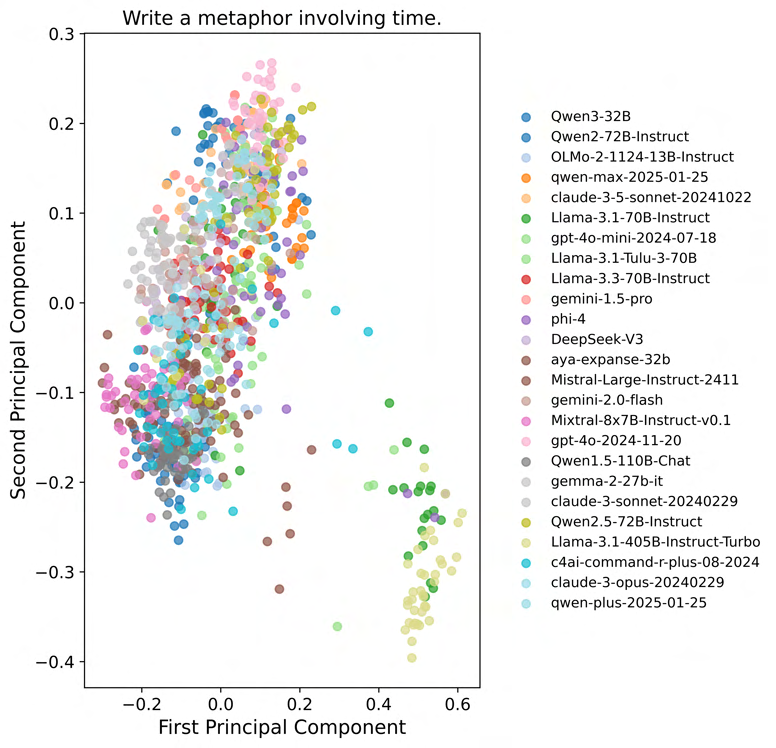
\includegraphics[width=\linewidth]{figures/hivemind.png}
  \caption{Distribution of final answer tokens across models and prompts. Each row is a model variant; columns are prompts and answer tokens are color-coded. Horizontal bars show the mean answer token distribution across all prompts; vertical bars show the model distribution across all prompts. \emph{Reproduced from} \cite{jiang2025hivemind}.}
  \label{fig:hivemind}
  \end{figure}

\section{Inference compute, theory, and memory efficiency}
Ellis-Mohr \emph{et al.}\ develop a theory of \emph{inference compute scaling}, casting test-time reasoning as search through a space of skills or procedures with a stochastic structure; that viewpoint links extra compute at inference to measurable gains in problem-solving when the search process is well aligned with the task \cite{ellis2026inference}. Independently of search theory, memory at inference remains a bottleneck for long contexts and long generations: Staniszewski and {\L}a\'{n}cucki propose transform coding for KV cache compression so stored activations remain usable while shrinking footprint \cite{staniszewski2026kv}. In short, scaling ``thinking time'' and scaling ``context memory'' are two levers that interact---cheapening the cache enables longer or wider inference processes within the same hardware budget.

\section{Robotics and lightweight human feedback}
Biyik surveys how robots can be trained from natural, low-burden human feedback---preferences, rankings, language corrections, and light interventions---rather than from full teleoperation trajectories alone \cite{biyik2025robots}. Such signals aim to improve sample efficiency and to match how non-expert users actually correct embodied agents in the field. The robotics perspective sharpens the themes from earlier sections: autonomy and reasoning must remain steerable under real-time and safety constraints, and lightweight supervision is often the only scalable way to align generalist policies with human intent.

\section{Discussion}
\begin{itemize}
    \item Compare tensions: scaling versus homogeneity; reasoning quality versus compute and memory; autonomy versus human oversight.
    \item List risks and research gaps suggested by the collected works.
\end{itemize}

\section{Conclusion}
\begin{itemize}
    \item Recap the cross-cutting themes and limitations of this short survey.
    \item Point to future reading directions beyond the nine sources.
\end{itemize}

\section*{Acknowledgment}
% Optional: funding, compute, colleagues. Remove if not needed.

\section*{References}

\begin{thebibliography}{00}

\bibitem{wang2025thousand}
K. Wang, I. Javali, M. Bortkiewicz, T. Trzci\'{n}ski, and B. Eysenbach, ``1000 Layer Networks for Self-Supervised RL: Scaling Depth Can Enable New Goal-Reaching Capabilities,'' 2026, arXiv:2503.14858. [Online]. Available: \url{https://arxiv.org/abs/2503.14858}

\bibitem{qiu2025gated}
Z. Qiu \emph{et al.}, ``Gated Attention for Large Language Models: Non-linearity, Sparsity, and Attention-Sink-Free,'' in \emph{Advances in Neural Information Processing Systems} (NeurIPS), 2025.

\bibitem{jiang2025hivemind}
L. Jiang \emph{et al.}, ``Artificial Hivemind: The Open-Ended Homogeneity of Language Models (and Beyond),'' in \emph{Advances in Neural Information Processing Systems} (NeurIPS), Datasets and Benchmarks Track, 2025.

\bibitem{sinha2025drcot}
A. Sinha, O. C. Umakanthan, and S. Gajendran, ``DR-CoT: Dynamic Recursive Chain of Thought With Meta Reasoning for Parameter Efficient Models,'' \emph{Sci. Rep.}, vol.~15, art.~34773, 2025, doi: 10.1038/s41598-025-18622-6.

\bibitem{ellis2026inference}
A. R. Ellis-Mohr, A. K. Nayak, and L. R. Varshney, ``A theory of inference compute scaling: Reasoning through directed stochastic skill search,'' \emph{Phil. Trans. R. Soc. A}, vol.~384, no.~20240510, 2026, doi: 10.1098/rsta.2024.0510.

\bibitem{staniszewski2026kv}
K. Staniszewski and A. {\L}a\'{n}cucki, ``KV Cache Transform Coding for Compact Storage in LLM Inference,'' 2026, arXiv:2511.01815. [Online]. Available: \url{https://arxiv.org/abs/2511.01815}

\bibitem{song2026mscot}
Z. Song, ``MS-CoT: Multi-scale chain-of-thought fusion for interpretable biological reasoning with large language models,'' \emph{Comput. Biol. Med.}, vol.~203, p.~111467, 2026, doi: 10.1016/j.compbiomed.2026.111467.

\bibitem{xu2025reasoning}
F. Xu, ``Toward large reasoning models: A survey of reinforced reasoning with large language models,'' \emph{Patterns}, vol.~6, no.~2, p.~101370, 2025, doi: 10.1016/j.patter.2025.101370.

\bibitem{biyik2025robots}
E. B{\i}y{\i}k, ``Training robots with natural and lightweight human feedback,'' \emph{AI Mag.}, 2025, doi: 10.1002/aaai.70037.

\end{thebibliography}

\end{document}
